\documentclass[12pt,a4paper]{report}

\usepackage[english]{babel}
\usepackage[cp1250]{inputenc} 
   % by u�y� polskich znak�w w systemach Linux
   % u�ywamy kodowania "latin2" lub "utf8", dla Windows "cp1250" 
\usepackage{graphicx}
\usepackage{gauss}
\usepackage{amsmath}
\usepackage{tikz}
\usepackage{float}


\newcommand*\circled[1]{\tikz[baseline=(char.base)]{
            \node[shape=circle,draw,inner sep=2pt] (char) {#1};}}
%-------------------------------------------------------------------------------
% TITLE PAGE
%-------------------------------------------------------------------------------

\begin{document}


\title{ \normalsize \textsc{Real Time Operating Systems}
        \\ [1.0cm]
        \line(1,0){350}
        \newline
      \LARGE \textbf  {Final Report}     \line(1,0){350}}
     \date{28.05.2018}
   
   \author{
        Wojciech Juszczak \\
        Jaros�aw Szumega\\
        Adam Superczy�ski }
        
\maketitle
\tableofcontents
\newpage

\newpage
\chapter{Introduction}
The aim of the project was building automatic, self-driving robot with ability to detect and avoid obstacles. System was implemented on STM32 with the use of FreeRTOS.
\newline
General architecture diagram of project is presented below.
\newline
\begin{figure}[h!]
  \caption{Architecture diagram}
  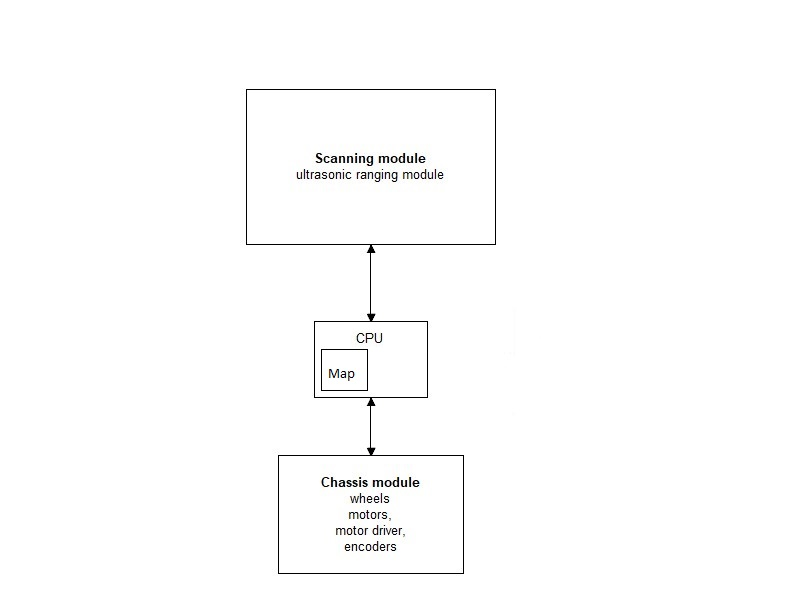
\includegraphics[width=1\textwidth]{architecture_diagram}
\end{figure}
\newline
The whole architecture can be divided into three elements:
\begin{itemize}
  \item Scanning module - used for surrounding scanning and informing about distance to obstacle,
  \item Map - information about surrounding stored inside CPU memory. Based on it robot makes decision about next movement,
  \item Chasis module - deciding about movement, controlling motors  \ldots
\end{itemize}
\chapter{Detailed description of project}
\section{Scanning module}
For this purpose proximity sensor HCSR-04 is used. To start measuring it needs 10us pulse on pin TRIG. After that it will response with pulse on ECHO pin which has width proportional to the distance. High priotity task activates measurement by clearing the timer and setting high signal on TRIG pin. Task becomes blocked and waits for interrupt from ISR. After 10us there is timer interrupt in which signal on TRIG pin is set to low. Next, values of timer in rising and falling edges are saved. On falling edge notification is sent to task. After receiving notification distance is calculated and saved to mutex - locked global variable. Task is blocked for 100ms before next measurement.

\newpage
\section{Map for constrained memory limit}
\subsection{Problem statement}
There is a necessity of having map stored in the robot memory. There is a few reasons of such an approach:
\begin{itemize}
	\item saving the scanning data aquired from sensors,
	\item having a structure that is easy to send and interpret on another device (e.g. for rendering 2D map on PC),
	\item introducing safety mechanisms (robot aware of obstacle ahead of it).
\end{itemize}
\noindent
The assumption was to have a map constructed of tiles (where one tile is more or less the surface covered by the robot -- ~ 30cm x 30cm).\\
\\
The problem was the storage -- if we need to cover room 10m x 10m, there is a need of having around 1200 cells representing each "tile", while the status of tile can one of four defined:
\begin{itemize}
	\item unknown,
	\item scanned and marked as obstacle,
	\item scanned and marked as free,
	\item marked as robot position.
\end{itemize}
\noindent
Using the array of integers is a waste of memory (which is also very limited in the arm processor).
\subsection{Solution}
To optimize the map, there was developed optimized C--code for memory access and manipulation. 
\\It takes advantage of bitwise operations, what drastically saves space (up to 16 times less memory is occupied by the map). There are four states, what means that each can be represented using only 2 bits in entire integer, therefore in 32--bit representation we get 16 states saved in one bit, in 16--bit, there can be stored 8 states, etc.
\newpage
\noindent
In the files \textbf{robot\_map.h}, \textbf{robot\_map.c} there are all necessary functions that were designed to deal with this optimized map storage (interpreted one--dimensional array as two--dimensional map where each integer  is seen as \textbf{sizeof(int)*8/2} cells for storing states).
\\
\\
Currently there is support for:
\begin{itemize}
	\item allocating map and basic operations on it,
	\item get/set the individual cells,
	\item setting n--cells ahead free, setting next cell free, setting next cell blocked, setting cell blocked at distance X,
	\item answering if the next cell is free (for robot safe movement),
	\item marking robot movements such as going forward, turning left, right and backwards.
\end{itemize}

There also a useful print function prepared for visual interpretation of optimized map -- it was used mainly for testing, but can be also an interface on PC computer to show the map.\\
It is simple and requires only knowledge of rows, columns and array -- therefore the data transfer is also very simple.

\begin{figure}[h]
\centering
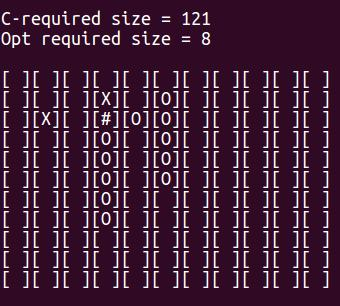
\includegraphics[width=0.5\linewidth]{map-example}
\caption{Example of map 11x11 cells}
(empty -- unknown, X -- obstacle, O -- free space,  -- rover position)
\label{fig:map-example}
\end{figure}

\end{document}